\documentclass{article} % Default font size and left-justified equations
% \documentclass{book}

\usepackage[
  margin=0.7in,
  % includefoot,
  % footskip=30pt,
]{geometry}
\usepackage{listings}
\usepackage{color}
\usepackage{natbib}
\usepackage{enumitem}
\usepackage{amsmath,amsfonts}
\usepackage{graphicx}
\usepackage{framed}
\usepackage{subcaption}
\usepackage[T1]{fontenc}%
\usepackage[utf8]{inputenc}%
\usepackage{mathrsfs}%
\usepackage{amssymb}%
\usepackage{amsthm}%
\usepackage{graphicx}
\usepackage{hyperref}
\usepackage{environ}
\usepackage{framed}
\usepackage{mdframed} 
\usepackage{wrapfig} 
\usepackage{booktabs}
\usepackage{tabularx} 
\usepackage{array}
\usepackage[font=small]{caption} 
\usepackage{xspace}  
\usepackage[osf,sc]{mathpazo}
\usepackage{pbox}
\usepackage{listings}
\usepackage{tikz}
\usepackage{bm}
\usepackage[strict]{changepage}
\usepackage{mleftright}
\usepackage{appendix}
\usepackage{wrapfig}
\usepackage[all]{xy} 
\setcounter{tocdepth}{3}
\setcounter{secnumdepth}{3}
% \usepackage[ruled,vlined]{algorithm2e}
\usepackage{algorithm}
\usepackage{algpseudocode}
\usepackage{framed}
\usepackage{wrapfig}
\usepackage{pythonhighlight}
\usepackage{tikz}
\usetikzlibrary{arrows}
\usetikzlibrary{arrows.meta}
\usetikzlibrary{shapes.geometric}
\usetikzlibrary{positioning, arrows, automata, calc}
\usepackage{transparent}
\usepackage[many]{tcolorbox}
\usepackage{tikz}
\usetikzlibrary{shapes.geometric}
\usetikzlibrary{positioning, arrows, automata, calc}

\newtcolorbox[]{your_solution}[1][]{
    % breakable,
    enhanced,
    nobeforeafter,
    colback=white,
    title=Your Answer,
    sidebyside align=top,
    box align=top,
    #1
}
\newcommand{\mybox}[1]{
\noindent
\fbox{\parbox{0.955\textwidth}{%
\noindent\texttt{#1}
}
}
}

\lstset{
    % backgroundcolor=\color{lightgray},   % choose the background color
    basicstyle=\ttfamily\small,          % font style
    frame=single,                        % add a frame around the code
    breaklines=true,                     % automatic line breaking
    captionpos=b,                        % position of the caption
    numbers=left,                        % where to put the line-numbers
    numberstyle=\tiny\color{gray},       % the style of the line numbers
    keywordstyle=\color{blue},           % keyword style
    commentstyle=\color{green},          % comment style
    stringstyle=\color{red},             % string literal style
}

\newcommand{\filler}{ . . . . . }
\newcommand{\choice}{\hspace{0.5cm}$\square$}
\newcommand{\identity}{\mathbf{I}} 
\newcommand{\paran}[1]{\left( #1 \right)}

%% PLEASE USE THESE MACROS WHEN WRITING THE SOLUTIONS 
\long\def\solution#1{\par\noindent{\color{purple}Answer: \em #1}\par} % show
%\newcommand{\solution}[2]{#2} % hide

\newcommand{\extracredit}{{\color{purple}\textbf{Extra Credit:}}}

\newcommand{\additionalNotes}{
\noindent\textbf{How to hand in your written work and code:} via Gradescope.  \\ 


% \noindent\textbf{Collaboration:} Make certain that you understand the course collaboration policy, described on the course website. 
% You may discuss the homework to understand the problems and the mathematics behind the various learning algorithms, but you are \textcolor{red}{\textbf{not allowed to share solutions with any other students. You must write the solutions \textbf{individually}}}. \\ 

% \noindent\textbf{Typesetting:} 
% We strongly recommend typesetting your homework, especially if you have sloppy handwriting! :)  
% % We recommend using LaTeX, but you are welcome to use whatever program and/or markup language you like. 
% We will provide a LaTeX template for homework solutions.
}

\newcommand{\additionalNotesTeamUpThree}{
\noindent\textbf{How to hand in your written work:} via Gradescope.  \\ 


\noindent\textbf{Collaboration:} 
You may discuss the homework with your classmates, if that helps you understand the problems and various ideas in the class, but you are \textcolor{red}{\textbf{not allowed to share problem solutions with any other students. You must write the solutions \textbf{individually}}. 
% You're not allowed to use AI for drafting responses.
The use of AI (e.g., Github CoPilot) is permitted but \textbf{must be documented}. 
} 
% Using AI for generating code (e.g., Github CoPilot) is permitted. 
\\ 

\noindent\textbf{Typesetting:} 
We strongly recommend typesetting your homework, especially if you have sloppy handwriting! :)  
% We recommend using LaTeX, but you are welcome to use whatever program and/or markup language you like. 
We will provide a LaTeX template for homework solutions.
Please be as succinct as possible in your answers; overly long responses will be penalized.

}

% \newcommand{\additionalNotesTeamUpThree}{
% \noindent\textbf{How to hand in your written work:} via Gradescope.  \\ 

\title{ \Large (CS 601.768) Language Model Agents }
\date{For homework deadline and collaboration policy, check the syllabus \\
\normalsize Name: Dev Vyas\_\_\_\_\   \\ 
% Collaborators, if any: \_\_\_\_\_\_\_\_\_\_\_\_\_\_\_\_\_\_\_\_\_\_\_\_\_\_\_\_\_\_\_\_\_\_\_\_\_\_\_\_\_\_\_\_\_\_\_\_\_\_\_\_ \\ 
Sources used for your homework, if any: \_\_\_\_\_\_\_\_\_\_\_\_\_\_\_\_\_\_\_\_\_\_\_\_\_\_\_\_\_\_\_\_\_\_\_\_\_\_\_\ 
}
\newcommand{\todo}{\textcolor{blue}{\textbf{TODOs}}}




\usepackage{macros}
\usepackage{float}
\usepackage{booktabs}

\author{
\Large
First (and Last) Homework
}

\begin{document}

\maketitle

This assignment will assess your understanding of foundational concepts in information retrieval, post-training, reinforcement learning, agent systems, and efficient language-model inference. \\
\\

\additionalNotesTeamUpThree


\section{Agent Loops and Inference Economics}

\subsection{Theory: Maintaining State in an Agent Loop}
Suppose an agent repeatedly takes an action, receives new information from its environment, and updates its internal belief state.
Consider three ways of constructing the model context at the next step:

\begin{enumerate}[label=(\alph*), itemsep=0.5ex]
    \item \textbf{Rewrite-state:} maintain a compact belief/state summary near the beginning of the prompt and rewrite that summary after every step.
    \item \textbf{Rewrite-suffix:} keep the earlier prefix fixed, but discard reasoning tokens that produced the previous action.
    \item \textbf{Append-only:} never rewrite previous context; append each new observation or state update to the end of the existing trajectory.
\end{enumerate}

Outline one advantage and one disadvantage for each approach. Consider factors such as context footprint, stale or contradictory information, ``\href{https://www.trychroma.com/research/context-rot}{context rot}'', human legibility, and inference efficiency where relevant.

\solution{\begin{enumerate}[label=(\alph*), itemsep=0.5ex]
    \item Rewrite-state: The main advantage is that the agent keeps a compact, up-to-date view of what matters, which helps control context growth and reduces stale information. The downside is that rewriting is lossy, so important details can get dropped or distorted, and changing an early part of the prompt can also reduce prompt-cache reuse.
    \item Rewrite-suffix: The advantage is that the agent can throw away old reasoning or tool-use traces that are no longer useful, so the context stays smaller while the stable prefix can still be cached. The downside is that some of that discarded reasoning may contain useful information about why a decision was made, and editing the suffix can also reduce cache continuity from that point onward.
    \item Append-only: The advantage is that it preserves the full trajectory and is usually the most cache-friendly approach because each new step simply extends the previous prompt. The downside is that the context keeps growing and can fill up with outdated, contradictory, or irrelevant information, which increases context rot and can make the model worse at focusing on the current state.
\end{enumerate}}


\subsection{Theory: KV Cache and Agent Design}
Why does the memory footprint of computing attention grow quadratically with context length?
Suppose an API charges cached input tokens at 0.1x the price of uncached input tokens. Which of the three agent designs above does this pricing structure most strongly incentivize, and why? Which design is least compatible with prefix caching?

\solution{In a conventional full-attention prefill, each of $L$ query positions interacts with $L$ key positions, making the attention-score matrix $L\times L$ (per head) and the attention work $O(L^2)$. Materializing that matrix also takes $O(L^2)$ temporary memory; FlashAttention-style kernels can avoid storing it all. The \emph{persistent KV cache} itself is $O(L)$ in sequence length for fixed model dimensions, not quadratic. That's an important distinction.

At 0.1x cached-input pricing, \textbf{append-only} is most attractive: yesterday's context is literally the prefix of today's, so it can be reused cheaply. \textbf{Rewrite-state} is least cache-friendly because modifying a summary near the start invalidates almost everything after it. Rewrite-suffix still preserves the unchanged earlier prefix, so it lands in the middle.}


\subsection{Empirical: Dense vs. Mixture-of-Experts Serving}
Using \textbf{vLLM} on a single GPU, investigate when a Mixture-of-Experts model provides a serving-throughput advantage over dense models.
Use the following three checkpoints:

\begin{center}
\begin{tabular}{lll}
\toprule
Checkpoint & Architecture & Role in comparison \\
\midrule
\texttt{allenai/OLMo-2-0425-1B-Instruct} & Dense & small dense baseline \\
\texttt{allenai/OLMoE-1B-7B-0924-Instruct} & MoE & $\sim$1B active / 7B total \\
\texttt{allenai/OLMo-2-1124-7B} & Dense & large dense baseline \\
\bottomrule
\end{tabular}
\end{center}

Serve all three models using \textbf{FP8 weights} and an \textbf{FP8 KV cache}.
Keep the serving setup otherwise as comparable as possible across models.

Design an experiment that separately characterizes \textbf{prefill-dominated} and \textbf{decode-dominated} workloads.
For prefill jobs, plot on the X axis the length of the input context and on the Y axis the average tokens/second. For decode jobs, plot the number of parallel generations on the X axis.
Your experiment should make it possible to understand the effects of model size, number of active parameters, sequence length, and concurrent decoding. Produce two figures that clearly summarize the prefill and decode results, alongside the raw measurements.

Then briefly interpret the results. Explain how the MoE behaves more like the small dense model and how it behaves more like the large dense model. You may reference the OLMoE technical report \citep{muennighoff2025olmoe} for more information about this model and its performance characteristics.

Include a pointer to the script in your code that implements this experiment.

\solution{\textbf{Setup.} I ran the three specified checkpoints one at a time on a single RTX 4070 SUPER with vLLM 0.30.0. Every model used online per-tensor FP8 weights, an FP8 KV cache, BF16 for unquantized tensors, eager execution, a 4096-token context limit, and disabled prefix caching. For prefill, the same deterministic technical passage was tokenized to 512, 1024, 2048, and 3000 body tokens; a short \texttt{yes} instruction followed it, and exactly one output token was forced. I measured prompt tokens divided by end-to-end request time, three repeats per length. For decode, the climate-essay prompt generated exactly 3000 tokens per request at parallelism 1, 2, and 4; I measured \emph{aggregate} generated tokens divided by batch wall time, twice per setting. Each point in the figures is the sample mean, with sample-standard-deviation bars.\par
\begin{center}\small
\begin{tabular}{lrrr}\toprule
Model & Prefill at 3000 body tokens & Decode $c=1$ & Decode $c=4$ \\\midrule
Dense 1B & 5,929 & 46.9 & 206.9 \\
MoE (1B active / 7B total) & 28,455 & 47.7 & 182.8 \\
Dense 7B & 1,576 & 11.6 & 32.4 \\\bottomrule
\end{tabular}\par
\emph{All rates are tokens/second; decode rates sum tokens across requests.}
\end{center}
\begin{figure}[H]\centering
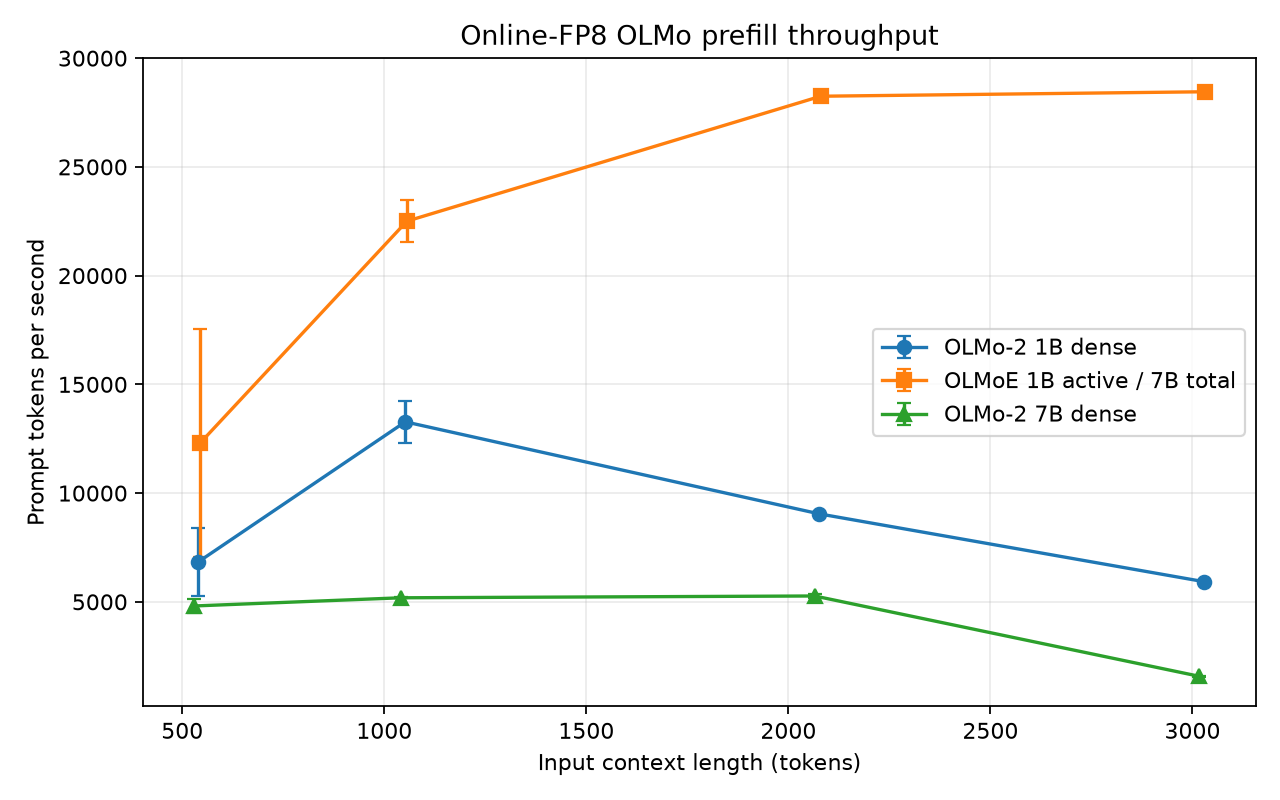
\includegraphics[width=.86\linewidth]{../results/q1_fp8_20260924_215129/prefill_throughput.png}
\caption{Prefill throughput versus input-context length (model-specific prompt wrappers add a few tokens).}
\end{figure}
\begin{figure}[H]\centering
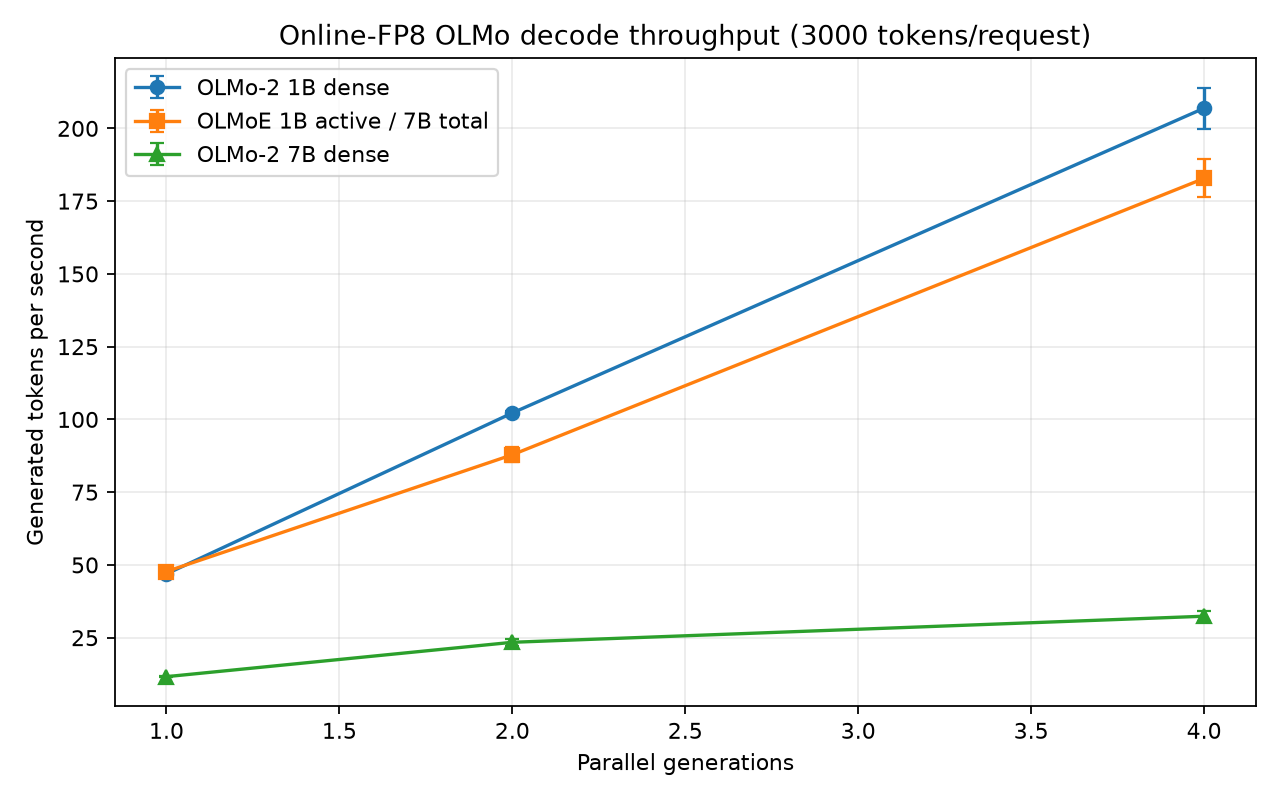
\includegraphics[width=.86\linewidth]{../results/q1_fp8_20260924_215129/decode_throughput.png}
\caption{Aggregate decode throughput versus concurrent generations.}
\end{figure}
\textbf{Reading the curves.} Here the MoE's decode speed is much closer to the small dense model than the 7B dense model: at four parallel requests it reaches 182.8 versus 206.9 and 32.4 tokens/s. That fits the idea that only a subset of experts runs per token. But it still has roughly 7B \emph{resident} parameters, so it is like the large model in weight-memory pressure; the engine reserved only about 3.11 GiB for its FP8 KV cache, versus 8.15 GiB for dense 1B. Interestingly, its measured prefill is \emph{faster than both} dense baselines at the longest context. I wouldn't sell that as a universal MoE law: FP8 expert kernels, routing, clock/JIT effects, and the unusually slow 7B long-context point all matter. Three prefill and two decode repeats are a small sample. The controlled inference setup is fair as a serving comparison, but model architecture is not the only moving part.\par
\textbf{Files on GitHub:} \href{https://github.com/SirNosh/LM-Agents-HW/blob/main/q3_benchmark.py}{benchmark code}; \href{https://github.com/SirNosh/LM-Agents-HW/blob/main/results/q1_fp8_20260924_215129/raw_measurements.csv}{raw measurements}; \href{https://github.com/SirNosh/LM-Agents-HW/blob/main/results/q1_fp8_20260924_215129/prefill_throughput.png}{prefill image}; \href{https://github.com/SirNosh/LM-Agents-HW/blob/main/results/q1_fp8_20260924_215129/decode_throughput.png}{decode image}.}



\section{Efficient Post-Training}

\subsection{Theory: LoRA Parameter and Memory Accounting}

Consider \texttt{Qwen/Qwen2.5-0.5B}, which has 24 transformer layers.
Suppose we apply LoRA \citep{hu2021lora} with $r=16$ to all linear transformations in each transformer
layer. These consist of the following seven projections:
\[
q_{\text{proj}},\ k_{\text{proj}},\ v_{\text{proj}},\ o_{\text{proj}},\
\text{gate}_{\text{proj}},\ \text{up}_{\text{proj}},\ \text{down}_{\text{proj}}.
\]

Their dimensions are:
\[
\begin{aligned}
q_{\text{proj}}, o_{\text{proj}} &: 896 \rightarrow 896,\\
k_{\text{proj}}, v_{\text{proj}} &: 896 \rightarrow 128,\\
\text{gate}_{\text{proj}}, \text{up}_{\text{proj}} &: 896 \rightarrow 4864,\\
\text{down}_{\text{proj}} &: 4864 \rightarrow 896.
\end{aligned}
\]

For a weight matrix
$W\in\mathbb{R}^{d_{\text{out}}\times d_{\text{in}}}$,
a rank-$r$ LoRA introduces matrices
\[
A\in\mathbb{R}^{r\times d_{\text{in}}},\qquad
B\in\mathbb{R}^{d_{\text{out}}\times r}.
\]

\begin{enumerate}[label=(\alph*), itemsep=0.5ex]
    \item How many trainable parameters does LoRA add to one
    transformer layer? To all 24 layers?

    \item Assuming trainable parameters and their gradients are both
    stored in 16-bit precision, how much memory is required to store
    the LoRA parameters and gradients? Ignore activations and optimizer
    state.

    \item For comparison, treat full fine-tuning as updating
    $0.49$ billion parameters. Under the same assumptions, how much
    memory is required for the full parameters and gradients?

    \item If AdamW \citep{loshchilov2017decoupled} additionally maintains two FP32 moment estimates for
    every trainable parameter, how does the comparison change?
    State any additional assumptions you make.
\end{enumerate}

You may validate your answer programmatically by constructing the
corresponding PEFT LoRA model and inspecting its number of trainable
parameters.

\solution{Each projection adds $r(d_{\rm in}+d_{\rm out})$ trainable parameters. Adding the seven projections in one layer gives
\[
16\bigl[2(896+896)+2(896+128)+3(896+4864)\bigr]
=\boxed{366{,}592}.
\]
Across 24 layers, that is $\boxed{8{,}798{,}208}$ parameters. At two bytes each for a parameter and its gradient, the LoRA total takes $4(8{,}798{,}208)=35{,}192{,}832$ bytes, or $\boxed{33.56\ \mathrm{MiB}}$. Updating 490 million full-model parameters under the same rule takes $1{,}960{,}000{,}000$ bytes, or $\boxed{1.825\ \mathrm{GiB}}$.\par
With two FP32 AdamW moments, add eight bytes per trained parameter, for twelve bytes each in total: LoRA becomes $105{,}578{,}496$ bytes ($\boxed{100.69\ \mathrm{MiB}}$), while full tuning becomes $5{,}880{,}000{,}000$ bytes ($\boxed{5.476\ \mathrm{GiB}}$). Full tuning is about $55.7\times$ larger under either assumption. These are just parameter/gradient/moment storage estimates; I exclude frozen base weights, activations, allocator overhead, possible FP32 master copies, and optimizer metadata. The actual PEFT rank-16 training run independently reported the same 8,798,208 trainable parameters.\par
\textbf{Files on GitHub:} \href{https://github.com/SirNosh/LM-Agents-HW/blob/main/q4_lora_accounting.py}{calculation code}; \href{https://github.com/SirNosh/LM-Agents-HW/blob/main/lora_accounting_results.txt}{raw text result}. No figure is needed for this arithmetic question.}


\subsection{Empirical: Supervised Fine-Tuning with LoRA}

Supervised fine-tune \texttt{Qwen/Qwen2.5-0.5B} using LoRA and full-weight fine-tuning. Apply LoRA to all linear layers in the
transformer using PEFT's
\texttt{target\_modules="all-linear"}.
Evaluate LoRA ranks in $\{1,4,16\}$, and full-weight tuning.

For training data, use the
\texttt{HuggingFaceH4/ultrachat\_200k} dataset, which contains
multi-turn conversations represented as sequences of user and assistant
messages. Select a fixed subset of 1000 conversations from
\texttt{train\_sft} for training and use examples from
\texttt{test\_sft} for held-out evaluation.

Keep the training setup as comparable as possible across LoRA ranks including the training examples, number of epochs, batch size, learning rate, and evaluation procedure.

Report:
\begin{itemize}
    \item the number of trainable parameters for each LoRA rank,
    \item the peak GPU memory utilization and training time at each rank,
    \item the training loss and validation loss over the course of
    training for each rank, and
    \item a small qualitative comparison of generations from the base
    model and each fine-tuned model on held-out user prompts.
\end{itemize}

Your qualitative examples should make it possible to assess whether
fine-tuning produced a meaningful change in the model's ability to
follow instructions and respond in a conversational format.
The goal is to demonstrate that you can construct an SFT pipeline,
apply parameter-efficient fine-tuning to a language model, and compare
the effect of LoRA rank; strong benchmark performance is not required.

Include a pointer to the script in your code that implements this experiment.

\solution{I trained \texttt{Qwen/Qwen2.5-0.5B} for one epoch on the \emph{saved} 1,000-conversation \texttt{train\_sft} subset (seed 42), masking non-assistant tokens. LoRA used PEFT \texttt{target\_modules="all-linear"} at ranks 1, 4, and 16; the fourth run updated all weights. All runs used BF16, 512-token truncation, batch size 1, gradient accumulation 8, and gradient checkpointing. The LoRA learning rate was $2\cdot10^{-4}$ for all ranks; full tuning used $2\cdot10^{-5}$. I also sampled 100 fixed conversations from \texttt{test\_sft} (seed 42, shuffle buffer 100; no overlap with the training subset), and apply the same assistant-only loss mask and final-512-token truncation for validation.\par
\begin{center}\small
\begin{tabular}{lrrrr}\toprule
Run & Trainable parameters & Time (s) & Peak allocated (GiB) & Last train loss \\\midrule
LoRA $r=1$ & 549,888 & 310.40 & 1.844 & 1.5673 \\
LoRA $r=4$ & 2,199,552 & 320.34 & 1.869 & 1.5520 \\
LoRA $r=16$ & 8,798,208 & 337.18 & 1.967 & 1.5471 \\
Full fine-tuning & 494,032,768 & 158.03 & 4.616 & 1.5436 \\\bottomrule
\end{tabular}
\end{center}
The ranks scale exactly as expected. In this implementation the full-weight run was actually faster despite using much more peak memory, so I would not generalize the wall-time ordering to other software/hardware. The loss column above is \emph{training} loss, and its last logged point is at step 120 (about epoch 0.96). The original run didn't save intermediate checkpoints, so I evaluated the saved final checkpoints rather than pretending to recover a training-time validation curve. Mean assistant-token cross-entropy on the identical 100 held-out conversations (42,477 target tokens) was: base $1.7732$, LoRA $r=1$ $1.6528$, $r=4$ $1.6375$, $r=16$ $1.6335$, and full FT $1.6274$ nats/token. All four tuned checkpoints are lower than the base on this sample; the gaps among tuned variants are much smaller than the gap from base. This is a single endpoint comparison on a 100-conversation subset, not a broad benchmark.\par
\begin{figure}[H]\centering
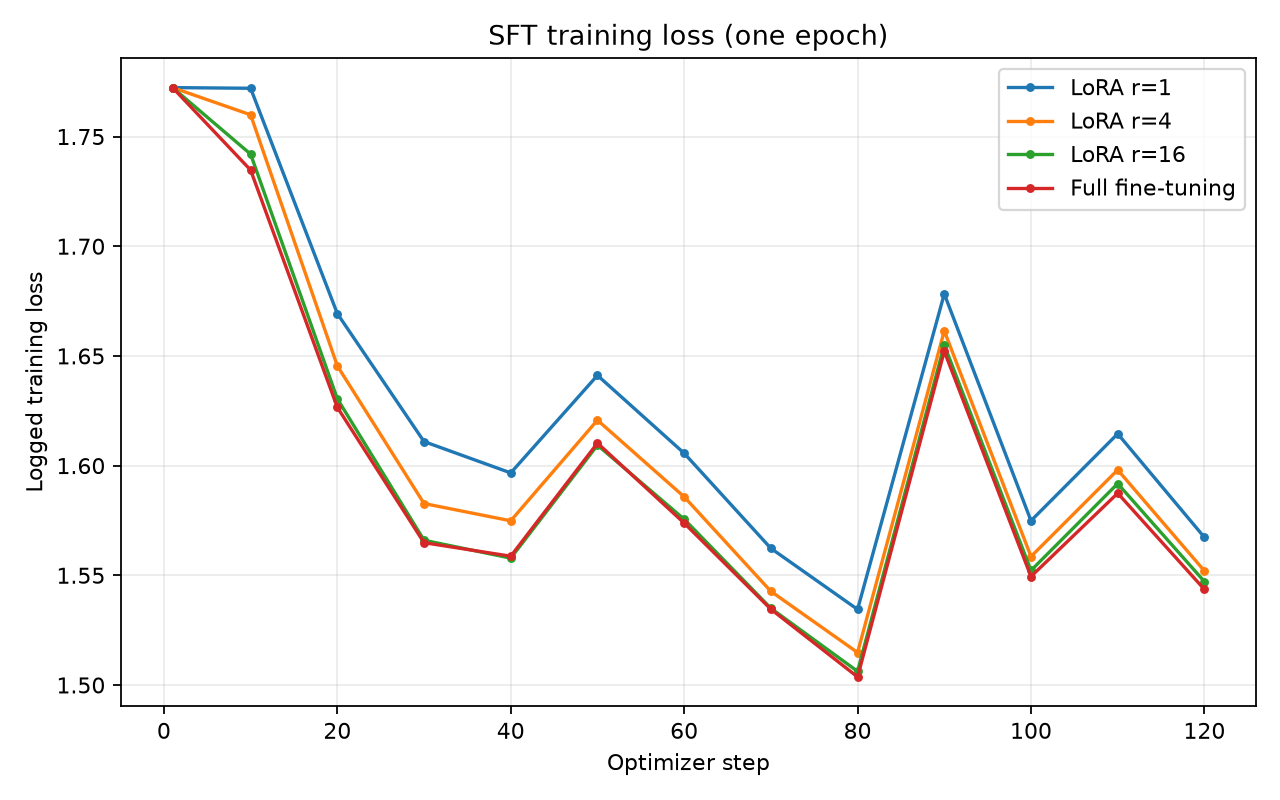
\includegraphics[width=.86\linewidth]{../results/sft_lora_20260924_204124/training_loss.png}
\caption{Logged training loss across the four one-epoch runs.}
\end{figure}
\begin{figure}[H]\centering
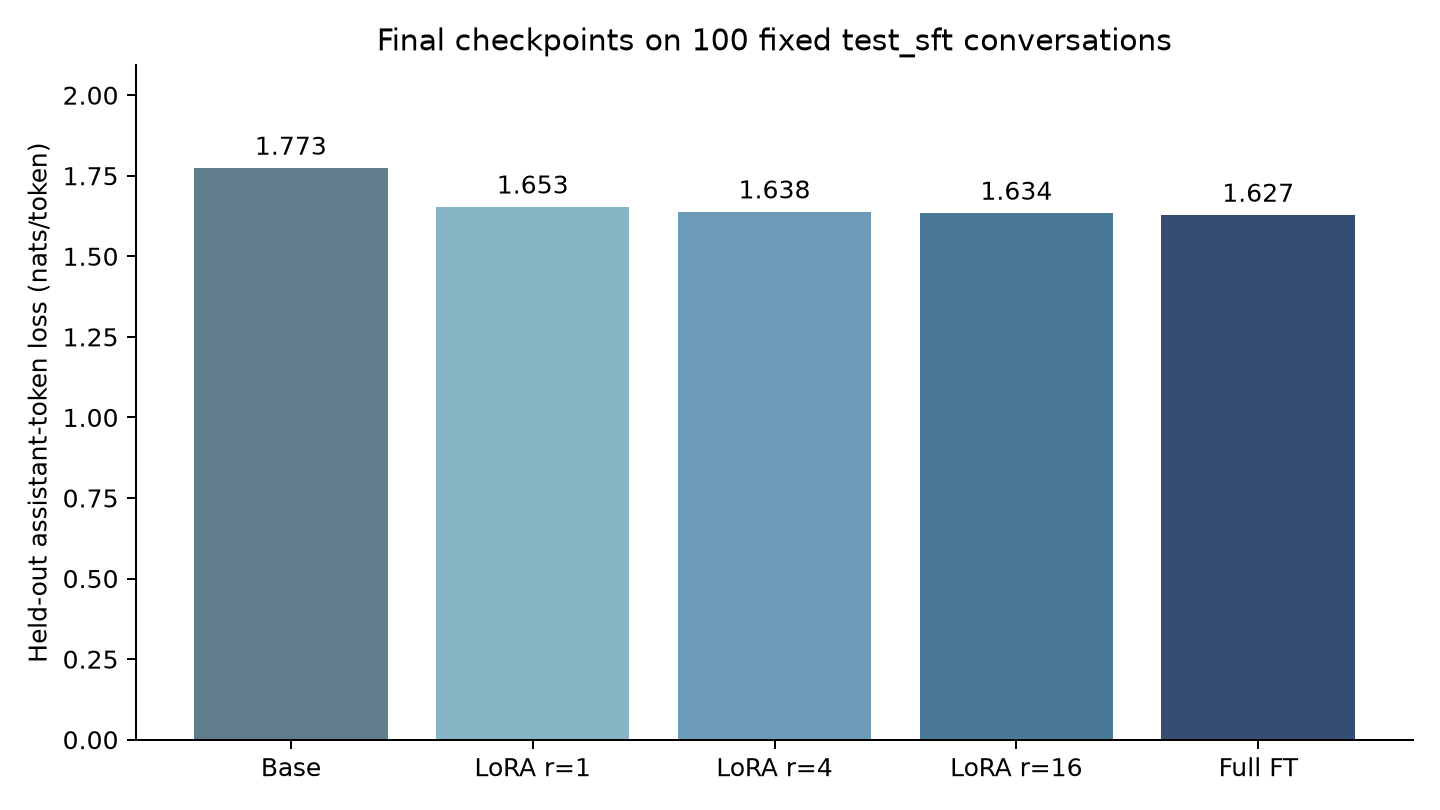
\includegraphics[width=.86\linewidth]{../results/sft_lora_20260924_204124/validation_loss.png}
\caption{Assistant-token loss on the same fixed 100-conversation test\_sft subset for the base model and saved final checkpoints.}
\end{figure}
The fixed subset contains lots of multi-turn follow-ups, numbered practical advice, and passage-based questions. To compare style and instruction-following, I used three \emph{new} prompts: a damaged-tool tracking plan, a clothing-swap follow-up with wheelchair-accessibility and a two-hour setup constraint, and a question grounded in a repair-cafe notice. Across these prompts, differences are mostly stylistic: $r=1$ is sometimes more orderly, $r=4$/$r=16$ add accessibility details but repeat or miss constraints, and full FT echoes the time limit without turning it into a schedule. All five models make the same core grounding error on the notice, so these three short generations show no reliable rank-by-rank improvement.\par
\textbf{Limit:} This is a final-checkpoint validation comparison on a fixed 100-conversation test\_sft subset, not the full test split. It does not show validation loss over training: the original training run saved no intermediate checkpoints. The qualitative prompts are separate from this quantitative subset.\par
\textbf{Files on GitHub:} \href{https://github.com/SirNosh/LM-Agents-HW/blob/main/q5_prepare_data.py}{subset code}; \href{https://github.com/SirNosh/LM-Agents-HW/blob/main/q5_sft_lora.py}{training code}; \href{https://github.com/SirNosh/LM-Agents-HW/blob/main/q5_qualitative.py}{generation code}; \href{https://github.com/SirNosh/LM-Agents-HW/blob/main/q5_validate.py}{validation code}; \href{https://github.com/SirNosh/LM-Agents-HW/blob/main/q5_plot_validation.py}{validation plotting code}; \href{https://github.com/SirNosh/LM-Agents-HW/blob/main/data/ultrachat_train_1000_seed42.jsonl}{exact training subset}; \href{https://github.com/SirNosh/LM-Agents-HW/blob/main/data/ultrachat_test_100_seed42.jsonl}{fixed held-out test subset}; \href{https://github.com/SirNosh/LM-Agents-HW/blob/main/results/sft_lora_20260924_204124/summary.csv}{raw summary}; \href{https://github.com/SirNosh/LM-Agents-HW/blob/main/results/sft_lora_20260924_204124/training_metrics.csv}{raw loss history}; \href{https://github.com/SirNosh/LM-Agents-HW/blob/main/results/sft_lora_20260924_204124/training_loss.png}{training-loss image}; \href{https://github.com/SirNosh/LM-Agents-HW/blob/main/results/sft_lora_20260924_204124/validation_summary.csv}{validation summary}; \href{https://github.com/SirNosh/LM-Agents-HW/blob/main/results/sft_lora_20260924_204124/validation_per_conversation.csv}{per-conversation validation results}; \href{https://github.com/SirNosh/LM-Agents-HW/blob/main/results/sft_lora_20260924_204124/validation_loss.png}{validation image}; \href{https://github.com/SirNosh/LM-Agents-HW/blob/main/results/sft_lora_20260924_204124/qualitative_comparison.txt}{side-by-side generations}; \href{https://github.com/SirNosh/LM-Agents-HW/blob/main/q5_subset_behavior_notes.txt}{qualitative interpretation notes}.}


\section{Language Model Reinforcement Learning}

\subsection{Theory: Formulating Language-Model Generation as RL}
Consider autoregressive generation from a language model.

\begin{itemize}
    \item Identify the \textbf{state}, \textbf{action}, \textbf{policy}, \textbf{transition function}, \textbf{reward}, and \textbf{trajectory} in this setting.
    \item Explain why the transition function is usually deterministic even though the policy is stochastic.
    \item Describe the difference between treating generation as an \textbf{MDP} and as a \textbf{contextual bandit}. When would each formulation be more natural? How does this distinction relate to outcome versus process rewards?
\end{itemize}

\solution{\begin{itemize}
    \item \textbf{State:} the prompt plus all tokens generated so far.
    \item \textbf{Action:} the next token the model chooses.
    \item \textbf{Policy:} the language model's probability distribution over the next token.
    \item \textbf{Transition:} append the chosen token to the current sequence.
    \item \textbf{Reward:} feedback on the generation, either after individual steps or at the end.
    \item \textbf{Trajectory:} the full sequence of states and generated tokens from the prompt to the final response.
\end{itemize}

The transition is usually deterministic because once a token is chosen, the next state is simply the old sequence with that token appended. The randomness comes from the policy deciding which token to choose, not from what happens after choosing it.

In an MDP, generation is treated as a sequence of decisions, usually one token or reasoning step at a time. This is more natural when intermediate decisions matter and we have process rewards. In a contextual bandit, the prompt is the context and the entire generated response is treated as one action that receives one reward. This is more natural for outcome rewards such as whether the final answer was correct or preferred. So, roughly: process rewards naturally fit the MDP view, while outcome-only rewards make the contextual-bandit view more natural. An MDP can still use only a final outcome reward.}


\subsection{Theory: REINFORCE and the Policy Gradient}
Describe the core training loop of \href{https://www.geeksforgeeks.org/machine-learning/reinforce-algorithm/}{\textbf{REINFORCE}}: what do we sample, what do we score, and what objective do we optimize?
Why is REINFORCE appealingly simple compared with actor--critic methods?
What is its central statistical weakness?

Explain why subtracting an action-independent baseline can change the variance of the policy-gradient estimator without changing its expectation.

\solution{REINFORCE samples a full trajectory from the current policy, assigns that trajectory a reward, and updates the model to make actions from high-reward trajectories more likely and actions from low-reward trajectories less likely. In the basic method, the reward directly weights the policy-gradient update.

REINFORCE is appealingly simple compared with actor--critic methods because it does not require a separate critic or value model; it uses the reward directly. Its main weakness is that the gradient estimate can be very noisy, leading to high variance and poor sample efficiency.

A baseline, such as the expected reward, can reduce variance by centering the return: the update depends on whether a trajectory did better or worse than the baseline. If the baseline is independent of the sampled action, subtracting it does not change the expected policy gradient, because its expected contribution cancels.} 


\subsection{Theory: Importance Sampling and Off-Policy Data}
Suppose rollouts were generated according to $\pi_{\text{old}}$, but we now want to optimize a different policy $\pi_\theta$.
Explain how importance sampling allows samples from one distribution to estimate an expectation under another distribution.
Why can importance ratios become problematic when the two policies differ substantially?
Explain the \textbf{bias--variance trade-off} introduced by clipping or truncating importance weights.

\solution{Importance sampling lets us reuse rollouts from $\pi_{\text{old}}$ by reweighting each sample based on how likely the new policy $\pi_\theta$ would have been to produce it. So samples that are more likely under the new policy count more, and samples that are less likely count less.

The problem is that if the two policies become very different, these ratios can become extremely large or small. A few trajectories can then dominate the update, giving us very high variance. This is especially an issue for LLMs because ratios can accumulate across many generated tokens.

Clipping or truncating the ratios limits how much any one sample can affect training. This lowers variance and makes training more stable, which is the basic idea behind methods like PPO. The trade-off is that once we modify those true ratios, the estimator becomes biased. So clipping basically trades some correctness in expectation for much more stable updates.}



\subsection{Theory: Proximal Policy Optimization}
PPO \citep{schulman2017proximal} updates a policy using the importance ratio
\[
r_t(\theta)=\frac{\pi_\theta(a_t\mid s_t)}{\pi_{\text{old}}(a_t\mid s_t)}.
\]

What does $r_t>1$ mean? What does $r_t<1$ mean?
Explain the role of \textbf{clipping} in the PPO objective.
What kind of update is clipping intended to prevent, and why might an unconstrained policy-gradient update be undesirable even when its estimated advantage has the correct sign?

\solution{If $r_t(\theta)>1$, the new policy assigns a higher probability to that action than the old policy did. If $r_t(\theta)<1$, it assigns a lower probability.

Clipping in PPO prevents the policy from benefiting from making that probability change too large. If an action has positive advantage, PPO encourages making it more likely, but only up to a point. If it has negative advantage, PPO encourages making it less likely, again only up to a point.

The goal is to prevent one update from moving the policy too far away from the policy that generated the data. Even if the advantage has the correct sign, its magnitude can be noisy or imperfect, so an unconstrained update could overreact and make the policy collapse or become unstable. PPO trades some aggressiveness for more stable updates.}


\subsection{Theory: Group Relative Policy Optimization}
GRPO \citep{shao2024deepseekmath} replaces a learned value-model baseline with a baseline estimated from multiple responses to the same prompt.
Suppose $G$ completions for one prompt receive rewards $r_1,\ldots,r_G$.
Write the standard group-relative advantage used by GRPO.

Then explain:
\begin{itemize}
    \item Why might a group-relative advantage be preferable to a learned critic?
    \item What additional cost does GRPO incur? On what types of types of tasks would GRPO be impossible to use?
    \item What happens when all responses in a group receive the same reward?
\end{itemize}

\solution{The standard GRPO advantage is
\[
\hat A_i = \frac{r_i - \bar r}{\sigma_r},
\qquad
\bar r = \frac{1}{G}\sum_{j=1}^{G} r_j,
\]
where $\sigma_r$ is the standard deviation of the rewards in the group. Each response is judged relative to the other responses generated for the same prompt.

A group-relative advantage can be preferable to a learned critic because it does not require training and maintaining a separate value model. The other sampled responses provide a baseline directly, saving model memory and avoiding errors from a poorly trained critic.

The extra cost is that multiple responses must be generated and scored for every prompt. This can be expensive, especially for long agent trajectories. GRPO is not really usable when the same situation cannot be reset and replayed multiple times, such as a one-shot real-world interaction where each action permanently changes the environment.

If every response receives the same reward, there is no relative signal within the group. After subtracting the mean, all advantages are zero, so the group provides no useful policy update. Implementations also need to handle the zero standard deviation numerically.}


\subsection{Theory: Modifications to GRPO}
Consider three modifications to vanilla GRPO discussed in the reading:

\begin{enumerate}
    \item \textbf{GSPO's sequence-level importance ratios},
    \item \textbf{DAPO's dynamic sampling},
    \item \textbf{Dr. GRPO's removal of response-length and question-difficulty biases}.
\end{enumerate}

Choose \textbf{two} and explain:
\begin{itemize}
    \item what failure mode of vanilla GRPO motivates the modification,
    \item how the proposed modification addresses that failure, and
    \item what new trade-off, if any, it introduces.
\end{itemize}

Your answer should focus on the mechanism rather than simply describing the algorithm.

\solution{I would choose DAPO dynamic sampling and Dr. GRPO.

\textbf{DAPO dynamic sampling:} In vanilla GRPO, if every response to a prompt gets the same reward, all of the relative advantages become zero. Compute is spent generating those responses, but they provide little or no learning signal. DAPO addresses this by dynamically resampling and retaining groups with reward variation, where at least some responses succeed and some fail. This makes training more efficient, but the trade-off is additional sampling cost and a bias toward prompts where the model has a mix of successes and failures. Very easy or extremely hard prompts may be filtered out more often.

\textbf{Dr. GRPO:} Vanilla GRPO normalizes by response length and by the reward variation within each question's group. This can create biases, such as penalizing long wrong answers less strongly and weighting questions differently depending on their reward variance. Dr. GRPO removes those normalization terms so updates more directly reflect whether a response did better or worse than the group average.

The trade-off is that removing length normalization means longer responses can contribute more total gradient simply because they contain more tokens. Recent work argues that this is a genuine trade-off: one can remove GRPO's original length bias, but cannot simultaneously make the estimator completely unbiased and completely independent of response length.}


\subsection{Theory: On-policy vs. Off-policy RL}
What is the distinction between \textbf{on-policy} and \textbf{off-policy} post-training?

Why might one prefer off-policy learning when high-reward trajectories are rare under the current policy?
Conversely, why might training on fresh samples from the current policy become valuable as the policy changes during training?


Explain how microbatches in PPO algorithms and stale rollouts in asynchronous RL systems blur the distinction between completely on-policy and off-policy learning.

\solution{On-policy post-training learns from trajectories generated by the current policy, while off-policy training uses trajectories generated by a different or older policy.

Off-policy learning is useful when good trajectories are very rare under the current model. Instead of waiting for the model to discover them, we can train on successful trajectories produced earlier, by another policy, or through search. The downside is distribution mismatch, because those trajectories may not reflect what the current model would actually do.

Fresh on-policy samples become valuable as the model improves because they show the states and mistakes the current model is actually encountering. Old data can become less relevant as the policy changes.

In practice, the distinction is blurry. PPO usually collects a rollout batch and then performs several minibatch updates on it. After the first few updates, that data was generated by an older version of the policy. Similarly, asynchronous RL systems may generate rollouts using slightly stale copies of the model while the learner keeps updating. Thus, many systems described as on-policy are approximately on-policy, with some controlled amount of policy lag.}

\subsection{Theory: RL for Agents}
The RL algorithms above mostly describe a single prompt followed by a single generated completion.
Explain what changes when the model instead interacts with an environment over many turns.

In particular, discuss:
\begin{itemize}
    \item why tool/environment outputs should generally be masked from the policy-gradient loss,
    \item why variable wall-clock trajectory lengths create an infrastructure problem that does not arise as strongly in ordinary single-turn RL, and
\end{itemize}

\solution{With an agent, the model is no longer generating one completion and stopping. It generates an action, gets an observation from a tool or environment, then continues for many turns. So the trajectory now mixes model-generated tokens with environment-generated tokens.

Tool/environment outputs should generally be masked from the policy-gradient loss because they are observations or results, not actions chosen by the model. The model-generated reasoning and tool calls around those observations are still trained, while the observations remain in context to influence later decisions.

The infrastructure also gets harder because trajectories can take very different amounts of time. One agent might finish after one quick tool call, while another waits on several searches or a slow code execution. If training waits for the whole batch to finish, GPUs can sit idle waiting for the slowest trajectory. This is why agent-RL systems increasingly implement asynchronous rollouts and load balancing, so completed trajectories can keep moving without being blocked by long-running ones.}

\section{Information Extraction and Retrieval}

\subsection{Theory: Sparse vs. Dense Retrieval}
What feature(s) of a query would lead you to expect a \textbf{sparse} retrieval system (e.g., BM25) to outperform a \textbf{dense} retrieval system (e.g., nearest-neighbor search over dense embeddings with FAISS)?
What features would lead you to expect better performance from a dense retriever?
Give at least one example query of each type and explain your reasoning.

When might a tool like \texttt{grep} be a better retrieval mechanism than BM25 or a dense embedding index?
When would it clearly be insufficient?


\solution{A sparse retriever like BM25 is usually better when the exact words matter, especially for rare terms, names, error codes, function names, or IDs. For example, a query like ``CVE-2024-3094'' should favor BM25 because the exact token is much more useful than semantic similarity. Dense retrieval is better when the query is about meaning and the relevant document may use different wording. For example, ``ways to reduce model hallucinations'' could retrieve documents discussing ``factuality'' or ``grounding'' even if they never use the word ``hallucination.''

\texttt{grep} can be even better when I already know the exact string, symbol, or pattern I am looking for, especially in a codebase. If I want every use of \texttt{process\_payment()} or a specific error message, grep is direct, exact, and does not require maintaining an index.

It becomes insufficient when I do not know the exact wording. For a query like ``where is authentication handled?'', the relevant code might contain \texttt{validate\_token} or \texttt{session\_manager} without ever saying ``authentication.'' In that case, semantic or indexed retrieval is much more useful.}


\subsection{Theory: Bi-Encoders vs. Cross-Encoders}
What is the architectural difference between a \textbf{bi-encoder} and a \textbf{cross-encoder}?
In a two-stage retrieval system consisting of \emph{retrieval} followed by \emph{reranking}, which architecture is better suited for each stage? Why?

\solution{A bi-encoder encodes the query and each document separately into embeddings, then compares those embeddings. Because document embeddings can be precomputed and indexed, it is very fast and works well for retrieving candidates from a huge corpus.

A cross-encoder takes the query and document together as one input and lets them directly attend to each other before producing a relevance score. That usually gives better relevance judgments, but it is much slower because the model must run separately for every query--document pair.

In a two-stage system:
\begin{itemize}
    \item \textbf{Retrieval:} use a bi-encoder, because it scales efficiently to millions of documents.
    \item \textbf{Reranking:} use a cross-encoder, because after retrieving only the top 50 or 100 candidates, the extra compute can be spent scoring them more accurately.
\end{itemize}}


\subsection{Theory: MapReduce over a Corpus}
This section considers questions asked about a corpus that is too large to fit into a language model's context window: all the emails exchanged within a fictional company OpenBrain.
For each question, describe how you could answer the question using a \textbf{MapReduce}-style procedure.

\begin{enumerate}
    \item What proportion of the emails within OpenBrain were sent to CEO Stan Allman?
    \item What proportion of the emails within OpenBrain discussed the cybersecurity capabilities of their most powerful model, Capricorn-6?
    \item Summarize all the emails Stan Allman received related to Capricorn-6's cybersecurity capabilities.
\end{enumerate}

In your answer, specify the logic of each map call, including its input and output specifications, alongside the logic of the reduce call(s) required. Consider that a language model query could be used for any of these calls, but will incur more computational cost than programmatic logic applied to a document's metadata.

\solution{\begin{enumerate}
    \item \textbf{Proportion of emails sent to Stan Allman}

    \textbf{Map:} For each email, inspect only the metadata and emit (\texttt{total}, 1). If Stan is a recipient, also emit (\texttt{to\_stan}, 1). No LLM is needed here.

    \textbf{Reduce:} Sum the values for \texttt{total} and \texttt{to\_stan}, then compute $\texttt{to\_stan}/\texttt{total}$.

    \item \textbf{Proportion discussing Capricorn-6 cybersecurity}

    \textbf{Map:} Give each email body to an LLM and ask whether it meaningfully discusses Capricorn-6's cybersecurity capabilities. Emit (\texttt{total}, 1) for every email and (\texttt{relevant}, 1) when the answer is yes.

    \textbf{Reduce:} Sum \texttt{relevant} and \texttt{total}, then compute $\texttt{relevant}/\texttt{total}$.

    \item \textbf{Summary of emails Stan received about Capricorn-6 cybersecurity}

    \textbf{Map:} First filter emails to Stan using metadata. Then give each of those emails to an LLM. If it is relevant to Capricorn-6 cybersecurity, emit (\texttt{capricorn\_cyber}, short summary).

    \textbf{Reduce:} Group all summaries under that key and combine them into one overall summary, removing repetition and preserving important details. If there are too many summaries to fit in context, perform the reduce hierarchically in multiple rounds.
\end{enumerate}}


\subsection{Theory: Comparing Retrieval Metrics}
Consider \textbf{Recall@$k$} and \textbf{Mean Reciprocal Rank (MRR)}.

\begin{itemize}
    \item Write the formula for each metric and explain in words what it measures.
    \item What are the best- and worst-case values for each metric?
    \item How do the two metrics differ in their sensitivity to the rank at which a relevant document appears?
    \item Give an example where two retrieval systems could have the same Recall@$k$ but different MRR. What does this tell you about the information captured by each metric?
\end{itemize}

\solution{\textbf{Recall@$k$:}
\[
\mathrm{Recall@}k = \frac{\text{number of relevant documents in the top }k}{\text{number of relevant documents overall}}.
\]
It measures how much of the relevant information the retriever finds within its top $k$ results. Its best value is 1 and worst is 0.

\textbf{Mean Reciprocal Rank (MRR):}
\[
\mathrm{MRR} = \frac{1}{N}\sum_{i=1}^{N}\frac{1}{\text{rank of the first relevant result for query }i}.
\]
It measures how quickly the user sees the first relevant result, averaged across queries. Its best value is 1, when a relevant result is always ranked first, and worst is 0, when no relevant result is retrieved.

The main difference is that Recall@$k$ mostly cares whether relevant documents appear somewhere within the top $k$, while MRR is very sensitive to where the first relevant result appears.

For example, suppose each query has one relevant document and $k=5$. System A ranks it at position 1, while System B ranks it at position 5. Both have Recall@5 = 1, but their reciprocal ranks are 1 and $1/5$. So Recall tells us whether we successfully retrieved the relevant information, while MRR also tells us how well we ranked the first useful result.}

\bibliographystyle{unsrtnat}
\bibliography{ref.bib}

\end{document}
